% A LaTeX template for EXECUTIVE SUMMARY of the MSc Thesis submissions to
% Politecnico di Milano (PoliMi) - School of Industrial and Information Engineering
%
% P. F. Antonietti, S. Bonetti, A. Gruttadauria, G. Mescolini, A. Zingaro
% e-mail: template-tesi-ingind@polimi.it
%
% Last Revision: October 2021
%
% Copyright 2021 Politecnico di Milano, Italy. Inc. All rights reserved.

\documentclass[11pt,a4paper]{article}

%------------------------------------------------------------------------------
%	REQUIRED PACKAGES AND  CONFIGURATIONS
%------------------------------------------------------------------------------
% PACKAGES FOR TITLES
\usepackage{titlesec}
\usepackage{color}

% PACKAGES FOR LANGUAGE AND FONT
\usepackage[utf8]{inputenc}
\usepackage[english]{babel}
\usepackage[T1]{fontenc} % Font encoding

% PACKAGES FOR IMAGES

\usepackage{subcaption}
\usepackage{graphicx}
\graphicspath{{Images/}} % Path for images' folder
\usepackage{eso-pic} % For the background picture on the title page
%\usepackage{subfig} % Numbered and caption subfigures using \subfloat
\usepackage{caption} % Coloured captions
\captionsetup[figure]{font=small}
\usepackage{transparent}
\usepackage{wrapfig}


% STANDARD MATH PACKAGES
\usepackage{amsmath}
\usepackage{amsthm}
\usepackage{amssymb}
\usepackage{bm}
\usepackage[overload]{empheq}  % For braced-style systems of equations

% PACKAGES FOR TABLES
\usepackage{tabularx}
\usepackage{longtable} % tables that can span several pages
\usepackage{colortbl}

% PACKAGES FOR ALGORITHMS (PSEUDO-CODE)
\usepackage{algorithm}
\usepackage{algorithmic}

% PACKAGES FOR REFERENCES & BIBLIOGRAPHY
\usepackage[colorlinks=true,linkcolor=black,anchorcolor=black,citecolor=black,filecolor=black,menucolor=black,runcolor=black,urlcolor=black]{hyperref} % Adds clickable links at references
\usepackage{cleveref}
\usepackage[square, numbers, sort&compress]{natbib} % Square brackets, citing references with numbers, citations sorted by appearance in the text and compressed
\bibliographystyle{plain} % You may use a different style adapted to your field

% PACKAGES FOR THE APPENDIX
\usepackage{appendix}

% PACKAGES FOR ITEMIZE & ENUMERATES
\usepackage{enumitem}

% OTHER PACKAGES
\usepackage{amsthm,thmtools,xcolor} % Coloured "Theorem"
\usepackage{comment} % Comment part of code
\usepackage{fancyhdr} % Fancy headers and footers
\usepackage{lipsum} % Insert dummy text
\usepackage{tcolorbox} % Create coloured boxes (e.g. the one for the key-words)
\usepackage{stfloats} % Correct position of the tables

%-------------------------------------------------------------------------
%	NEW COMMANDS DEFINED
%-------------------------------------------------------------------------
% EXAMPLES OF NEW COMMANDS -> here you see how to define new commands
\newcommand{\bea}{\begin{eqnarray}} % Shortcut for equation arrays
\newcommand{\eea}{\end{eqnarray}}
\newcommand{\e}[1]{\times 10^{#1}}  % Powers of 10 notation
\newcommand{\mathbbm}[1]{\text{\usefont{U}{bbm}{m}{n}#1}} % From mathbbm.sty
\newcommand{\pdev}[2]{\frac{\partial#1}{\partial#2}}
\newcommand{\tinyline}{\vspace{-0.5em} {\setlength{\baselineskip}{0.8\baselineskip} \textcolor{white}{..........} }\\ }

% NB: you can also override some existing commands with the keyword \renewcommand

%----------------------------------------------------------------------------
%	ADD YOUR PACKAGES (be careful of package interaction)
%----------------------------------------------------------------------------
\usepackage{exscale}
\DeclareMathSizes{10}{11}{10}{10}
% \makeatletter
% \renewcommand\everydisplay{\textstyle\@math@crampedtrue}
% \makeatother
%----------------------------------------------------------------------------
%	ADD YOUR DEFINITIONS AND COMMANDS (be careful of existing commands)
%----------------------------------------------------------------------------


% Do not change Configuration_files/config.tex file unless you really know what you are doing.
% This file ends the configuration procedures (e.g. customizing commands, definition of new commands)
% Set the geometric layout of the document
\usepackage{geometry}
\geometry{
  top=3cm,
  left = 2.0cm,
  right = 2.0cm,
  bottom=2cm,
  headheight= 2cm,
  headsep= 0cm,
}
\raggedbottom

% Create color bluePoli (-> manuale grafica coordinata:  https://www.polimi.it/fileadmin/user_upload/il_Politecnico/grafica-coordinata/2015_05_11_46xy_manuale_grafica_coordinata.pdf)
\definecolor{bluePoli}{cmyk}{0.4,0.1,0,0.4}

% Custom theorem environments
\declaretheoremstyle[
  shaded={rulecolor=bluePoli!20, rulewidth=1pt, bgcolor=bluePoli!5},
  headfont=\color{bluePoli}\normalfont\bfseries,
  bodyfont=\color{black}\normalfont,
]{colored}

\captionsetup[figure]{labelfont={color=bluePoli}} % Set colour of the captions
\captionsetup[table]{labelfont={color=bluePoli}} % Set colour of the captions
\captionsetup[algorithm]{labelfont={color=bluePoli}} % Set colour of the captions

\theoremstyle{colored}
\newtheorem{theorem}{Theorem}[section]
\newtheorem{proposition}{Proposition}[section]
\newtheorem{definition}{Definition}[section]
\newtheorem*{remark}{Remark}
\newtheorem{lemma}{Lemma}[section]

% Enhances the features of the standard "table" and "tabular" environments.
\newcommand\T{\rule{0pt}{2.6ex}}
\newcommand\B{\rule[-1.2ex]{0pt}{0pt}}

% Algorithm description
\newcounter{algsubstate}
\renewcommand{\thealgsubstate}{\alph{algsubstate}}
\newenvironment{algsubstates}{
    \setcounter{algsubstate}{0}%
    \renewcommand{\STATE}{%
    \stepcounter{algsubstate}%
    \Statex {\small\thealgsubstate:}\space}
    }{}

% Custom theorem environment
\newcolumntype{L}[1]{>{\raggedright\let\newline\\\arraybackslash\hspace{0pt}}m{#1}}
\newcolumntype{C}[1]{>{\centering\let\newline\\\arraybackslash\hspace{0pt}}m{#1}}
\newcolumntype{R}[1]{>{\raggedleft\let\newline\\\arraybackslash\hspace{0pt}}m{#1}}

% Custom itemize environment
\setlist[itemize,1]{label=$\bullet$}
\setlist[itemize,2]{label=$\circ$}
\setlist[itemize,3]{label=$-$}
\setlist{nosep}

% Set separation of columns
\setlength{\columnsep}{30pt}

% Create command for background pic
\newcommand\BackgroundPic{% Adding background picture
	\put(230,358){
		\parbox[b][\paperheight]{\paperwidth}{%
			\vfill
			\centering
			\transparent{0.2}
			
\includegraphics[width=0.8\paperwidth]{raggiera_polimi.eps}%
			\vfill
}}}

% Set indentation
%\setlength\parindent{0pt}

% Custom title commands
\titleformat{\section}
{\color{bluePoli}\normalfont\Large\bfseries}
{\color{bluePoli}\thesection.}{1em}{}
\titlespacing*{\section}
{0pt}{2ex}{1ex}

\titleformat{\subsection}
{\color{bluePoli}\normalfont\large\bfseries}
{\color{bluePoli}\thesubsection.}{1em}{}
\titlespacing*{\subsection}
{0pt}{2ex}{1ex}

\titleformat{\subsubsection}
{\color{bluePoli}\normalfont\normalsize\bfseries}
{\color{bluePoli}\thesubsubsection.}{1em}{}
\titlespacing*{\subsubsection}
{0pt}{2ex}{1ex}

% Custom headers and footers
\pagestyle{fancy}
\fancyhf{}

\fancyfoot{}
\fancyfoot[C]{\thepage} % page
\renewcommand{\headrulewidth}{0mm} % headrule width
\renewcommand{\footrulewidth}{0mm} % footrule width

\makeatletter
\patchcmd{\headrule}{\hrule}{\color{black}\hrule}{}{} % headrule
\patchcmd{\footrule}{\hrule}{\color{black}\hrule}{}{} % footrule
\makeatother

% -> Create the header
\chead[C]{
\centering
\begin{tcolorbox}[arc=0pt, boxrule=0pt, colback=bluePoli!60, width=\textwidth, colupper=white]
    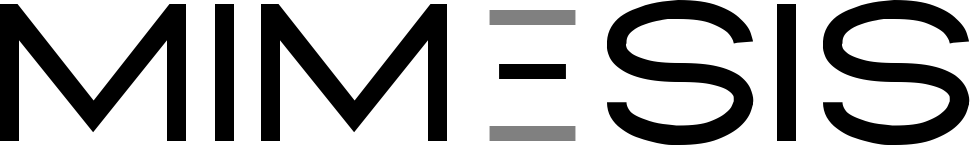
\includegraphics[width=0.2\textwidth]{mimesis.png}
\end{tcolorbox}
}


% Insert here the info that will be displayed into your Title page
% -> title of your work
\renewcommand{\title}{Uncertainty Quantification in Scientific Machine Learning}

% -> author name and surname
\renewcommand{\author}{Andrea Bonifacio}
% -> MSc course
\newcommand\norm[1]{\lVert#1\rVert}
\newcommand{\course}{Numerical Analysis for Partial Differential Equations}
% -> advisor name and surname
%\newcommand{\advisor}{Dr. Stefano Pagani}
% IF AND ONLY IF you need to modify the co-supervisors you also have to modify the file Configuration_files/title_page.tex (ONLY where it is marked)
%\newcommand{\firstcoadvisor}{Name Surname} % insert if any otherwise comment
%\newcommand{\secondcoadvisor}{Name Surname} % insert if any otherwise comment
% -> academic year
\newcommand{\YEAR}{2022-2023}

%-------------------------------------------------------------------------
%	BEGIN OF YOUR DOCUMENT
%-------------------------------------------------------------------------
\begin{document}

%-----------------------------------------------------------------------------
% TITLE PAGE
%-----------------------------------------------------------------------------
% Do not change Configuration_files/TitlePage.tex (Modify it IF AND ONLY IF you need to add or delete the Co-advisors)
% This file creates the Title Page of the document
% DO NOT REMOVE SPACES BETWEEN LINES!

%\twocolumn[{\begin{@twocolumnfalse}

\AddToShipoutPicture*{\BackgroundPic}

\hspace{-0.6cm}
\includegraphics[width=0.6\textwidth]{logo_polimi_ing_indinf.eps}

\vspace{-1mm}
\fontsize{0.3cm}{0.5cm}\selectfont \bfseries \textsc{\color{bluePoli} Report}\\

\vspace{-0.2cm}
\Large{\textbf{\color{bluePoli}{\title}}}\\

\vspace{-0.2cm}
\fontsize{0.3cm}{0.5cm}\selectfont \bfseries \textsc{\color{bluePoli} \course}\\

\vspace{-0.2cm}
\fontsize{0.3cm}{0.5cm} \selectfont \bfseries Authors: \textsc{\textbf{\author}}\\

%\vspace{-0.4cm}
%\fontsize{0.3cm}{0.5cm}\selectfont \bfseries Advisor: \textsc{\textbf{\advisor}}\\

% if only ONE co-advisor is present:
%\vspace{-0.4cm}
%\fontsize{0.3cm}{0.5cm}\selectfont \bfseries Co-advisor: \textsc{\textbf{\firstcoadvisor}}\\
% if more than one co-advisors are present:
%\vspace{-0.4cm}
%\fontsize{0.3cm}{0.5cm}\selectfont \bfseries Co-advisors: \textsc{\textbf{\firstcoadvisor}}\textsc{\textbf{\secondcoadvisor}}\\

\vspace{-0.4cm}
\fontsize{0.3cm}{0.5cm}\selectfont \bfseries Academic year: \textsc{\textbf{\YEAR}}

\small \normalfont

\vspace{11pt}

\centerline{\rule{1.0\textwidth}{0.4pt}}

%\vspace{15pt}
%\end{@twocolumnfalse}}]

\thispagestyle{plain} % In order to not show the header in the first page


%%%%%%%%%%%%%%%%%%%%%%%%%%%%%%
%%     THESIS MAIN TEXT     %%
%%%%%%%%%%%%%%%%%%%%%%%%%%%%%%

%-----------------------------------------------------------------------------
% INTRODUCTION
%-----------------------------------------------------------------------------
\section{Introduction}
In this report I'll try to review the main Uncertainty Quantification (UQ) methods in Neural Networks (NNs), with a focus on Physics Informed Neural Networks (PINNs). To do so, I'll present a brief recap on UQ and NNs, followed by the methodology to quantify uncertainty while solving SDEs using PINNs. \cite{bibtex}
\subsection{Neural Networks}
Today NNs are all over the news, they are the tools behind many new inventions, like large language models. Here I'll describe the simplest possible architecture for a neural network. 

In its most basic configuration, a feed-forward neural network is made up of three layers:
\begin{itemize}
    \item Input layer,
    \item Hidden layer,
    \item Output layer.
\end{itemize}
While the first and last layers are quite self-explanatory (the input layer takes a vector \(\bm{x}\) \(D\)-dimensional as an input and the output layer returns an object compatible with the dimensions of the dataset), the hidden layer is made up of multiple units, called neurons, which are basically vector transformations, to which is applied a nonlinear function. The general idea behind is to minimize the loss between the predictions of the model and the real values of the training dataset, by continuously modifying the neurons. Once a satisfying loss between the prediction and real results is reached, the model is ready to be used. 

One of the main features of NNs is that they work really well as function approximators, so one of the logical step after their introduction was to use them to solve PDEs, Lagaris et al 1998, but, at the time, it didn't lead anywhere until recently, when the advent of new tools and machine learning frameworks made possible to work again on solving PDEs using neural networks built up for the task.
\subsection{Uncertainty Quantification}
To describe uncertainty in a model, we must distinguish between the two different kinds. The model itself cannot represent reality as a whole, it will always be built up on assumptions that adds up creating epistemic uncertainty, which must be acknowledged, as it is irreducible. In the real world, data are collected by humans and sensors, which are both prone to errors and noise. This is the second kind of uncertainty, called aleatoric. To sum up, the total uncertainty in a model is made of two components:
\[
    \text{TU} = \text{EU} + \text{AU}.
\]

To deal with epistemic uncertainty, it is possible to use a probability distribution over the model parameters. Given a dataset \(D = \left\{ \bm{x}_i, y_i \right\}^N_{i=1}\) where \(\bm{x}_i \in \mathbb{R}^D\) are the inputs and \(y_i \in \left\{ 1,\ldots, C \right\}\) are the corresponding outputs in \(C\) different classes. The idea is to optimize the parameters \(\omega\) of a function \(y = f^\omega(\bm{x})\). The Bayesian approach defines a model likelihood \(p(y\vert\bm{x}, \omega)\), from which we can obtain the posterior distribution for a given dataset, thanks to Bayes' theorem:
\[
    p(\omega \vert X, Y) = \frac{p(Y\vert X, \omega)p(\omega)}{p(Y\vert X)}.
\]
Now, given a test sample \(\bm{x}^*\), a class label can be predicted as 
\[
    p(y^*\vert \bm{x}^*, X, Y) = \int p(y^*\vert\bm{x}^*, \omega) p(\omega \vert X, Y) \, d\omega.
\]

\section{Problem setup}
The problem can be formulated in the following way
\begin{equation}
    \begin{cases}
        \mathcal{N}_x\left[ u(x;\omega); k(x;\omega) \right], & x \in \mathcal{D}, \omega \in \Omega, \\
        \mathcal{B}_x\left[ u(x;\omega) \right] = 0, & x \in \Gamma,
    \end{cases}
    \label{problem_setup}
\end{equation}
where \(\mathcal{N}_x\) is a differential operator, \(\mathcal{D}\) the domain, \(\Omega\) the random space and \(u(x;\omega)\) the solution. On the boundary \(\Gamma\) we have the boundary conditions imposed by the operator \(\mathcal{B}_x\). \(k(x;\omega)\) represent the random parameter.

There are two possible problems: 
\begin{itemize}
    \item Forward problems: in this case, we know the distribution of \(k(x;\omega)\) everywhere on the domain, and the quantity of interest is \(u(x;\omega)\).
    \item Inverse problems: when the information about \(k(x;\omega)\) is partially known, but there is a lot more information about \(u(x;\omega)\) it is possible to infer the full distribution of \(k\).
\end{itemize}

\section{Methodology}
\subsection{PINNs for deterministic systems}
Here is how to solve differential equations using PINNs. To do so, \eqref{problem_setup} must be rewritten replacing the random inputs with a set of finite parameters, to transform it in a deterministic problem.
\begin{equation}
    \begin{cases}
        \mathcal{N}_x\left[ u; \eta \right], & x \in \mathcal{D}, \\
        \mathcal{B}_x\left[ u \right] = 0, & x \in \Gamma.
    \end{cases}
    \label{problem_setup_det}
\end{equation}
The neural network will be denoted by \(\hat{u}(x;\theta)\), which is the approximation of the solution \(u(x)\) with a specific set of parameters \(\theta\) dependent on the network. In a classical deep learning setting, the network should have one constraint, which is to reproduce the values in the dataset. In a physics informed settings, there is a second constraint, which is that the network should comply with the physical laws imposed by \eqref{problem_setup_det}. 

To do so, a second network is defined 
\begin{equation}
    \hat{f}(x;\theta,\eta) := \mathcal{N}_x\left[ \hat{u}(x;\theta);\eta \right],
    \label{second_network}
\end{equation}
which is computed straightforwardly from \(\hat{u}\). The parameters of the second network are the same of the first one. 
Assuming a dataset with \(N_u\) observations on \(u\) collected at \(\{ x^{(i)}_u \}^{N_u}_{i=1}\) and \(N_c\) the number of collocation point in which \(\hat{f}\) will be evaluated.
\begin{algorithm}[H]
\caption{PINN for solving differential equations}\label{alg:cap}
\textbf{Step 1:} Specify the training set 
\[
    \hat{u}: \{ (x^{(i)}_u, u(x^{(i)}_u))\}^{N_u}_{i=1}, \quad \hat{f} = \{x^{(i)}_f, 0\}^{N_c}_{i=1}.
\]
\textbf{Step 2:} Construct a NN \(\hat{u}(x;\theta)\) with random initialized parameters \(\theta\). \\
\textbf{Step 3:} By using automatic differentiation, construct the residual network \(\hat{f}(x;\theta, \eta)\). \\
\textbf{Step 4:} Specify a loss function that includes both networks 
\begin{equation}
    \label{loss_fn}
    \mathcal{L}(\theta, \eta) = \frac{1}{N_u} \sum_{i=1}^{N_u} [\hat{u}(x^{(i)}_u; \theta) - u(x^{(i)}_u)]^2+ \frac{1}{N_c} \sum_{i=1}^{N_c}\hat{f}(x_f^{(i)};\theta, \eta)^2.
\end{equation}
\textbf{Step 5:} Train the networks to find the best parameters by minimizing the loss function:
\[
    \theta = \arg \min \mathcal{L}(\theta,\eta)
\]
\end{algorithm}
\subsection{Moving to a stochastic setting}
The idea now is to analyze a stochastic problem, which brings back \eqref{problem_setup}. A new dataset is needed to collect all the random events. This dataset will be made up of \(N_k\) measurement at \(x^{(i)}_k\) locations in the domain. Given \(N\) measurements, the random instance at the \(s^{\text{th}}\) event will be called \(\omega_s\). Now, defining \(k_s^{(i)} = k(x_k^{(i)}; \omega_s)\) and \(u_s^{(i)} = u(x_u^{(i)};\omega_s)\), the new dataset is built up like this:
\[
    \mathcal{S}_t = \{\{(x^{(i)}_k, k^{(i)}_s)\}^{N_k}_{i=1},\{(x^{(i)}_u, u^{(i)}_s)\}^{N_u}_{i=1},\{(x^{(i)}_f,0)\}^{N_f}_{i=1}\}^{N}_{s=1}.
\]    
The next step is the arbitrary polynomial chaos (aPC) expansion, which will require:
\begin{enumerate}
    \item Dimension reduction;
    \item Constructing the aPC basis;
    \item Building the NN-aPC network as a surrogate model and train the network for each mode.
\end{enumerate}
\subsubsection{Dimension reduction with PCA}
To find a lower dimensional space, the proposed technique is principal component analysis (PCA), which finds a smaller number of modes able to explain almost all the dataset with enough accuracy. In this case, the reduced dataset will be the one about \(k\).
Let \(K\) be the \(N_k\times N_k\) covariance matrix of the measurements on \(k\)
\[
   K_{i,j} = \text{Cov}(k^{(i)}, k^{(j)}).
\]
Given \(\lambda_l\) and \(\phi_l\) be the \(l\)-largest eigenvalue and its eigenvector, it is possible to write 
\[
    K = \bm{\Phi}^T\bm{\Lambda}\bm{\Phi},
\]
where \(\bm{\Phi} = \phi_1, \phi_2 \ldots, \phi_{N_k}\) is an orthonormal matrix and \(\bm{\Lambda} = \text{diag}(\lambda_1, \lambda_2, \ldots, \lambda_{N_k})\) is a diagonal matrix. 
%-----------------------------------------------------------------------------
% NUMERICAL RESULTS
%-----------------------------------------------------------------------------
 \section{Numerical Results}
%-----------------------------------------------------------------------------
% CONCLUSION
%-----------------------------------------------------------------------------
\section{Conclusions}

%---------------------------------------------------------------------------
%  BIBLIOGRAPHY
%---------------------------------------------------------------------------
% Remember to insert here only the essential bibliography of your work
\bibliography{bibliography.bib} % automatically inserted and ordered with this command

\end{document}